\begin{frame}[allowframebreaks]{WaveNet}
    % --- Causal Convolution ---
    \begin{columns}
        \begin{column}{0.6\linewidth}
            \begin{figure}
                \centering
                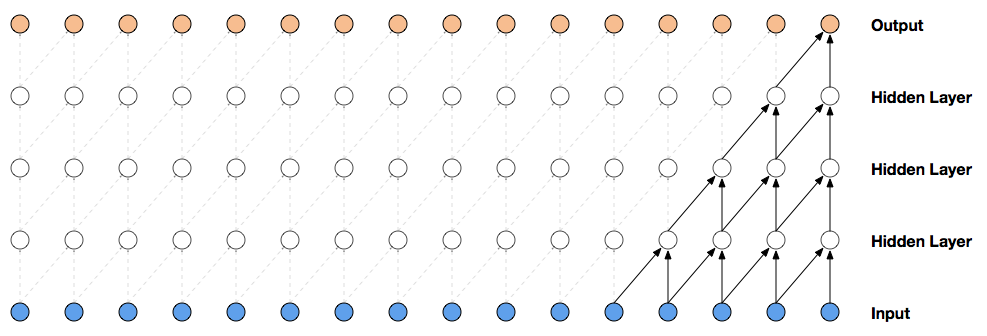
\includegraphics[width=1\linewidth]{images/autoregressive/casual-convolution.png}
                \caption*{Visualization of a stack of causal convolutional layers.}
            \end{figure}
        \end{column}
        \begin{column}{0.5\linewidth}
            \begin{itemize}
                \item \textbf{Causal convolution:} Each output depends only on current and previous inputs.
                \item Easy to implement: masking part of the convolution kernel.
                \item Constant parameter count for variable-length distributions.
                \item Efficient to compute: convolution has hyper-optimized implementations on all hardware.
                \item[] \textbf{However:}
                \begin{itemize}
                    \item Limited receptive field, grows linearly with the number of layers.
                \end{itemize}
            \end{itemize}
        \end{column}
    \end{columns}
    \small [WaveNet – Van den Oord et al, 2016]

    \framebreak

    % --- Softmax Output Distribution ---
    \textbf{Softmax Output Distribution}

    \begin{itemize}
        \item WaveNet models the conditional distribution of the next sample as a categorical distribution:
    \end{itemize}
    \begin{equation*}
        p(x_t | x_{1}, \ldots, x_{t-1}) = \mathrm{Softmax}(f(x_{1}, \ldots, x_{t-1}))
    \end{equation*}
    \begin{itemize}
        \item The output at each timestep is a probability distribution over possible quantized values.
        \item Typically, 8-bit $\mu$-law quantization is used for audio.
    \end{itemize}

    \framebreak

    % --- Dilated Convolutions ---
    \begin{columns}
        \begin{column}{0.6\linewidth}
            \begin{figure}
                \centering
                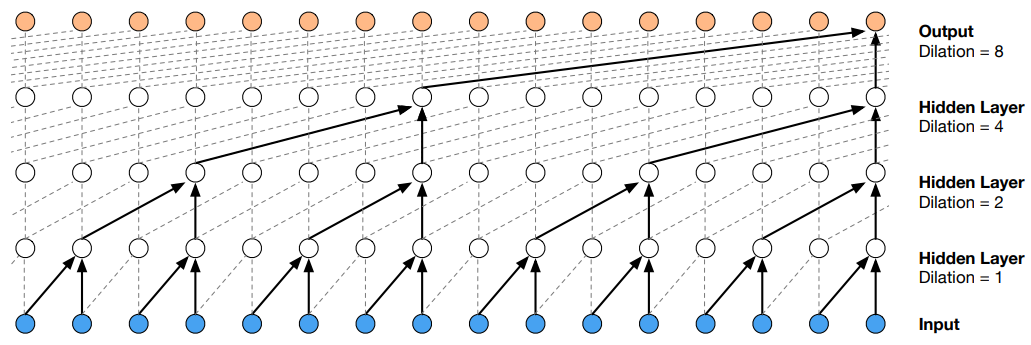
\includegraphics[width=1\linewidth]{images/autoregressive/dilated-casual-convolution.png}
                \caption*{Visualization of a stack of \textit{dilated} causal convolutional layers.}
            \end{figure}
        \end{column}
        \begin{column}{0.5\linewidth}
            \begin{itemize}
                \item \textbf{Dilated convolution:} Expands receptive field exponentially with depth.
                \item Dilation factor $d$:
                \begin{equation*}
                    y[t] = \sum_{k=0}^{K-1} w[k] \cdot x[t - d \cdot k]
                \end{equation*}
                \item Enables efficient modeling of long-range dependencies.
            \end{itemize}
        \end{column}
    \end{columns}
    \small [WaveNet – Van den Oord et al, 2016]

    \framebreak

    % --- Gated Activation Units ---
    \textbf{Gated Activation Units}

    \begin{itemize}
        \item Each residual block uses gated activation units:
    \end{itemize}
    \begin{equation*}
        z = \tanh(W_{f} * x) \odot \sigma(W_{g} * x)
    \end{equation*}
    \begin{itemize}
        \item $W_{f}$, $W_{g}$: convolution filters for filter and gate.
        \item $\odot$: element-wise multiplication.
        \item $\sigma$: sigmoid activation.
        \item Improves expressivity and helps gradient flow.
    \end{itemize}

    \framebreak

    % --- Residual and Skip Connections ---
    \textbf{Residual and Skip Connections}

    \begin{columns}
        \begin{column}{0.6\linewidth}
            \begin{figure}
                \centering
                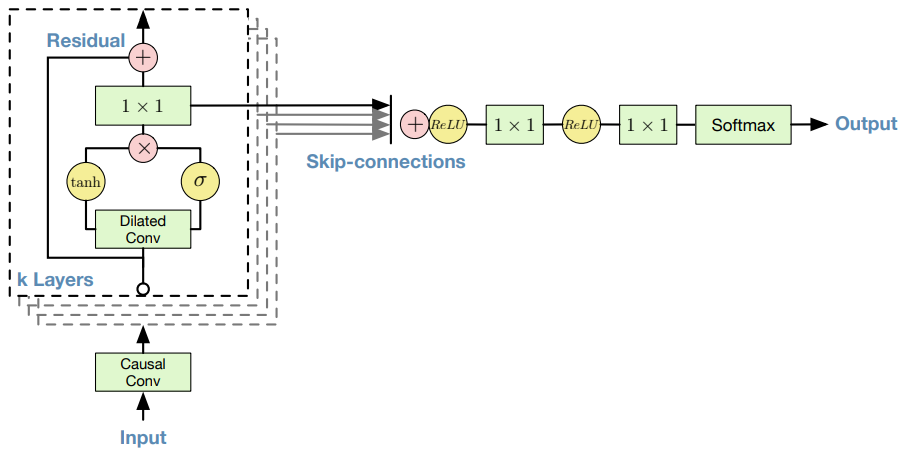
\includegraphics[width=1\linewidth]{images/autoregressive/architecture-residual-block.png}
                \caption*{Overview of the residual block and the entire architecture.}
            \end{figure}
        \end{column}
        \begin{column}{0.5\linewidth}
            \begin{itemize}
                \item \textbf{Residual connections:} Add input to output of each block.
                \item \textbf{Skip connections:} Aggregate outputs from all blocks before final output.
                \item Helps training deep networks and improves convergence.
            \end{itemize}
        \end{column}
    \end{columns}

    \framebreak

    % --- Conditional WaveNet ---
    \textbf{Conditional WaveNet}

    \begin{itemize}
        \item WaveNet can be conditioned on additional information (e.g., speaker identity, linguistic features).
        \item Conditioning vector $h$ is added to each layer:
    \end{itemize}
    \begin{equation*}
        z = \tanh(W_{f} * x + V_{f} * h) \odot \sigma(W_{g} * x + V_{g} * h)
    \end{equation*}
    \begin{itemize}
        \item Enables applications like text-to-speech (TTS) and voice conversion.
    \end{itemize}

    \framebreak

    % --- Context Stacks ---
    \textbf{Context Stacks}

    \begin{itemize}
        \item Multiple stacks of dilated convolutions with different dilation rates.
        \item Each stack captures dependencies at different temporal scales.
        \item Improves model's ability to capture both short-term and long-term context.
    \end{itemize}
    \begin{equation*}
        \text{Stack}_i: \quad d \in \{1, 2, 4, \ldots, 2^{n-1}\}
    \end{equation*}

    \framebreak

    \textbf{\large WaveNet on MNIST}
    \vspace{2em}
    \begin{columns}
        \begin{column}{0.18\linewidth}
            \begin{figure}
                \centering
                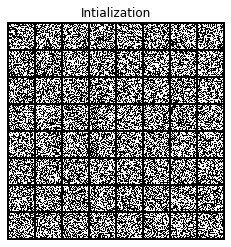
\includegraphics[width=1\linewidth]{images/autoregressive/mnist/init.png}
            \end{figure}
        \end{column}
        \begin{column}{0.18\linewidth}
            \begin{figure}
                \centering
                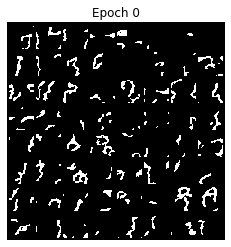
\includegraphics[width=1\linewidth]{images/autoregressive/mnist/epoch-0.png}
            \end{figure}
        \end{column}
        \begin{column}{0.18\linewidth}
            \begin{figure}
                \centering
                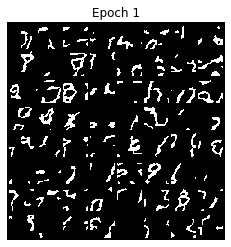
\includegraphics[width=1\linewidth]{images/autoregressive/mnist/epoch-1.png}
            \end{figure}
        \end{column}
        \begin{column}{0.18\linewidth}
            \begin{figure}
                \centering
                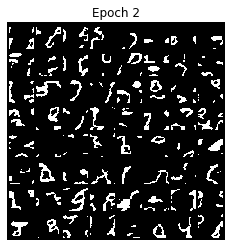
\includegraphics[width=1\linewidth]{images/autoregressive/mnist/epoch-2.png}
            \end{figure}
        \end{column}
        \begin{column}{0.18\linewidth}
            \begin{figure}
                \centering
                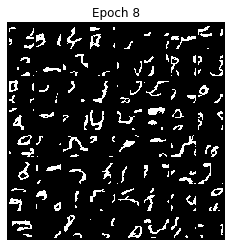
\includegraphics[width=1\linewidth]{images/autoregressive/mnist/epoch-8.png}
            \end{figure}
        \end{column}
        \begin{column}{0.18\linewidth}
            \begin{figure}
                \centering
                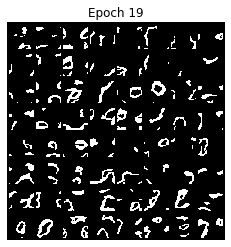
\includegraphics[width=1\linewidth]{images/autoregressive/mnist/epoch-19.png}
            \end{figure}
        \end{column}
    \end{columns}

    \framebreak

    \textbf{\large WaveNet with Pixel Location Appended on MNIST} \\
    \vspace{2em}
    Append (x,y) coordinates of pixel in the image as input to WaveNet
    \vspace{1em}
    \begin{columns}
        \begin{column}{0.18\linewidth}
            \begin{figure}
                \centering
                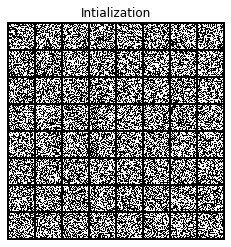
\includegraphics[width=1\linewidth]{images/autoregressive/mnist/init.png}
            \end{figure}
        \end{column}
        \begin{column}{0.18\linewidth}
            \begin{figure}
                \centering
                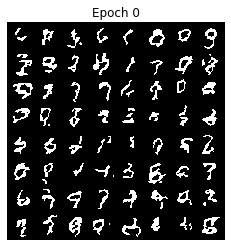
\includegraphics[width=1\linewidth]{images/autoregressive/mnist/coord-epoch-0.png}
            \end{figure}
        \end{column}
        \begin{column}{0.18\linewidth}
            \begin{figure}
                \centering
                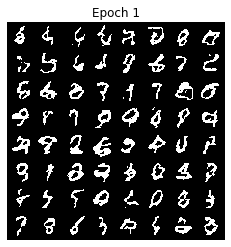
\includegraphics[width=1\linewidth]{images/autoregressive/mnist/coord-epoch-1.png}
            \end{figure}
        \end{column}
        \begin{column}{0.18\linewidth}
            \begin{figure}
                \centering
                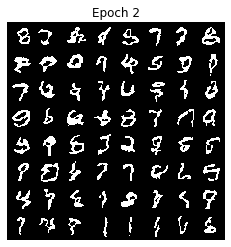
\includegraphics[width=1\linewidth]{images/autoregressive/mnist/coord-epoch-2.png}
            \end{figure}
        \end{column}
        \begin{column}{0.18\linewidth}
            \begin{figure}
                \centering
                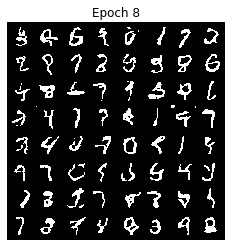
\includegraphics[width=1\linewidth]{images/autoregressive/mnist/coord-epoch-8.png}
            \end{figure}
        \end{column}
        \begin{column}{0.18\linewidth}
            \begin{figure}
                \centering
                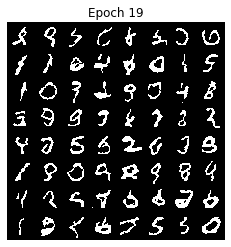
\includegraphics[width=1\linewidth]{images/autoregressive/mnist/coord-epoch-19.png}
            \end{figure}
        \end{column}
    \end{columns}

    \framebreak

    % --- Summary ---
    \textbf{WaveNet} is a deep generative model for raw audio waveforms, introduced by DeepMind in 2016. It models the conditional probability of the next audio sample given all previous samples using stacks of causal, dilated convolutional layers.

    \begin{itemize}
        \item \textbf{Autoregressive}: Predicts each audio sample sequentially, conditioning on previous samples.
        \item \textbf{Dilated Convolutions}: Enables the model to capture long-range temporal dependencies efficiently.
        \item \textbf{Gated Units, Residual/Skip Connections}: Improve expressivity and trainability.
        \item \textbf{Conditional WaveNet}: Allows conditioning on external features.
        \item \textbf{Applications}: High-quality text-to-speech (TTS), music generation, and audio synthesis.
        \item \textbf{Advantages}: Produces highly realistic and natural-sounding audio compared to previous methods.
    \end{itemize}
\end{frame}